\section{Cell Envelope Biogenesis}
We next turn to the processes that build and maintain the cell envelope. In
contrast to nutrient transporters, which support the synthesis of biomolecules
throughout the cell and therefore need to scale with the cell size, here we must
consider the synthesis of components that will need to scale with the surface
area of the cell, namely the synthesis of lipids and peptidoglycan. \textit{E.
coli} is a rod-shaped bacterium with a remarkably robust length-to-width aspect
ratio of $\approx$ 4:1 \citep{harris2018, ojkic2019}. At modest growth rates,
the total cell surface area is $\approx$ 5 \textmu m$^2$ (BNID: 101792,
\cite{milo2010}). Assuming this surface area is approximately the same between
the inner and outer membranes of \textit{E. coli}, and the fact that each
membrane is itself a lipid bilayer, cells have a the total membrane surface area
of $\approx 20$\textmu m$^2$. In Appendix \nameref{protein_size_SV} we describe
the calculation of cell surface area as a function of cell size.




% The carbon transported across the membrane is incorporated into nearly every
% biological molecule synthesized by the cell and, as we will see, many of these
% synthesis requirements scale with the cell volume. One unique exception is in
% the synthesis of components of the cell envelope -- namely the synthesis of
% lipids and peptidoglycan -- which define the cell surface area. Given our
% conclusion that expression of the carbon transporters could be increased to
% avert rate limiting transport, we will now explore some of the key processes
% dedicated to building this membrane real estate.

\subsection{Lipid Synthesis}

% The cell envelopes of gram negative bacteria (such as \textit{E. coli}) are
% composed of inner and outer phospholipid bilayer membranes separated by a
% $\approx 10$ nm periplasmic space (BNID: 100016).

% While this represents the total area of the membrane, this does not mean that it
% is composed entirely of lipid molecules. Rather,

The dense packing of the membrane with proteins means that the cell membranes
are not composed entirely of lipid molecules, with  only $\approx$ 40 \% of the
membrane area is occupied by lipids (BNID: 100078). Using a rule-of-thumb of 0.5
nm$^2$ as the surface area of the typical lipid (BNID: 106993), we can
estimate $\sim$ 2 $\times$ 10$^7$ lipids per cell, which is in close
agreement with experimental measurements (BNID: 100071, 102996).

The membranes of \textit{E. coli} are composed of a variety of different lipids,
each of which are unique in their structures and biosynthetic pathways
\citep{sohlenkamp2016}. Recently, a combination of stochastic kinetic modeling
\citep{ruppe2018} and \textit{in vitro} kinetic measurements
\citep{ranganathan2012, yu2011} have revealed remarkably slow steps in the fatty
acid synthesis pathways which may serve as the rate limiting reactions. One such
step is the removal of hydroxyl groups from the fatty-acid chain by ACP
dehydratase that leads to the formation of carbon-carbon double bonds. This
reaction, catalyzed by proteins FabZ and FabA in \textit{E. coli}
\citep{yu2011}, have been estimated to have kinetic turnover rates of $\approx$
1 dehydration per second per enzyme \citep{ruppe2018}. Thus, given this rate and
the need to synthesize $\approx$ 2 $\times$ 10$^7$ lipids over 5000 seconds, one
can estimate that a typical cell requires $\approx$ 4000 ACP dehydratases. This
is in reasonable agreement with the experimentally observed copy numbers of FabZ
and FabA (\FIG{cell_envelope}(A)). Furthermore, we can extend this estimate to
account for the change in membrane surface area as a function of the growth rate
(grey line in \FIG{cell_envelope}(A)), which captures the observed growth rate
dependent expression of these two enzymes.


\subsection{Peptidoglycan Synthesis}
Bacterial cells demonstrate exquisite control over their cell shape. This is
primarily due to the cell wall, a stiff, several nanometer thick meshwork of
polymerized discaccharides. The formation of the peptidoglycan is an intricate
process involving many macromolecular players \citep{shi2018, morgenstein2015},
whose coordinated action maintains cell shape and integrity even in the face of
large-scale perturbations \citep{harris2018,shi2018}.
The peptidoglycan alone comprises $\approx$ 3\% of the cellular dry mass (BNID:
101936), making it the most massive molecule in \textit{E. coli}. The
polymerized unit of the peptidoglycan is a N-acetylglucosamine and
N-acetylmuramic acid disaccharide, of which the former is functionalized with a
short pentapeptide. With a mass of $\approx$ 1000 Da, this unit, which we refer
to as a murein monomer, it is polymerized to form long strands in the periplasm
which are then attached to each other via their peptide linkers. Together, these
quantities provide an estimate of $\approx$ 5 $\times$ 10$^6$ murein monomers
per cell.

% While variation in cell size can vary substantially across growth conditions,

% interspersed with short peptide crosslinks termed the peptidoglycan. The cell
% wall is also a vital structural component that counteracts turgor pressure. In
% \textit{E. coli}, this enormous peptidoglycan molecule is a few nanometers thick
% and resides within the periplasmic space between the inner and outer membrane.

% , and can
% restore rod-shaped morphology even after digestion of the peptidoglycan

% At our archetypal growth rate,

The crosslinking of the pentapeptides between adjacent glycan strands is
repsonsible for maintaining the structural integrity of the cell wall and, in
principle, each murein monomer can be involved in such a crosslink. In some
microbes, such as in gram-positive bacterium \textit{Staphylococcus aureus},
the extent of crosslinking can be large with $>$ 90\% of pentapeptides
forming a connection between glycan strands. In \textit{E. coli}, however, a
much smaller proportion ($\approx$ 20\%) of the peptides are crosslinked,
resulting in a weaker and more porous cell wall \cite{vollmer2008a,
rogers1980}. The formation of these crosslinks occurs primarily during the
polymerization of the murein monomers and is facilitated by a family of
enzymes called transpeptidases. The four primary transpeptidases of
\textit{E. coli} have only recently been quantitatively characterized
\textit{in vivo} via liquid chromatography mass spectrometry
\citep{catherwood2020}, which revealed a notably slow kinetic turnover rate
of $\approx 2$ crosslinking reactions formed per second per enzyme.

Assembling these quantities permits us to make an estimate that on the order of
$\approx$ 100 transpeptidases per cell are needed for complete maturation of the
peptidoglycan, given a division time of $\approx$ 5000 seconds; a value that is
comparable to experimental observations (\FIG{cell_envelope}(B)). Expanding this
estimate to account for the changing mass of the peptidoglycan as a function
of growth rate (grey line in \FIG{cell_envelope}(B)) also qualitatively captures
the observed dependence in the data, though systematic disagreements between the
different data sets makes the comparison more difficult.

\subsubsection{Limits on Cell Wall Biogenesis}

While the processes we have considered represent only a small portion of
proteins devoted to cell wall biogenesis, we find it unlikely that they limting
cellular growth in general. The relative amount of mass required for lipid and
peptidoglycan components decrease at faster growth rates due to a decrease in
their surface area to volume (S/V) ratio \citep{ojkic2019}. In addition, despite the slow catalytic
rate of FabZ and FabA in lipid synthesis, experimental data and recent
computational model has shown that the rate of fatty-acid synthesis can be
drastically increased by increasing the concentration of FabZ \citep{yu2011,
ruppe2018}. With a proteome size of $\approx$ 3$\times$10$^6$ proteins, a
hypothetical 10-fold increase in expression from 4000 to 40,000 ACP dehydratases
would result in a $\approx$ 1\% increase in the size of the proteome.

% we find it unlikely that
% the generation of fatty acids would be a bottleneck in cell division and is
% not the key process responsible for setting the bacterial growth rate.

% Much as in the case of fatty acid synthesis, we find it unlikely that the
% formation of peptidoglycan is a process which defines the rate of bacterial
% cell division. The estimate we have presented considered only the
% transpeptidase enzymes that are involved lateral and longitudinal elongation
% of the peptidoglycan. This neglects the presence of other transpeptidases
% that are present in the periplasm and also involved in remodeling and
% maturation of the peptidoglycan. It is therefore possible that if this was
% setting the speed limit for cell division, the simple expression of more
% transpeptidases may be sufficient to maintain the structural integrity of the
% cell wall.
%
% As many other proteins are in much
% larger abundance than 4000 per cell (as we will see in the coming sections),
% it is unlikely that expression of ACP dehydratases couldn't be increased to
% speed up lipid synthesis and thereby facilitate faster growth.



\begin{figure}
    \begin{fullwidth}
    \centering{
    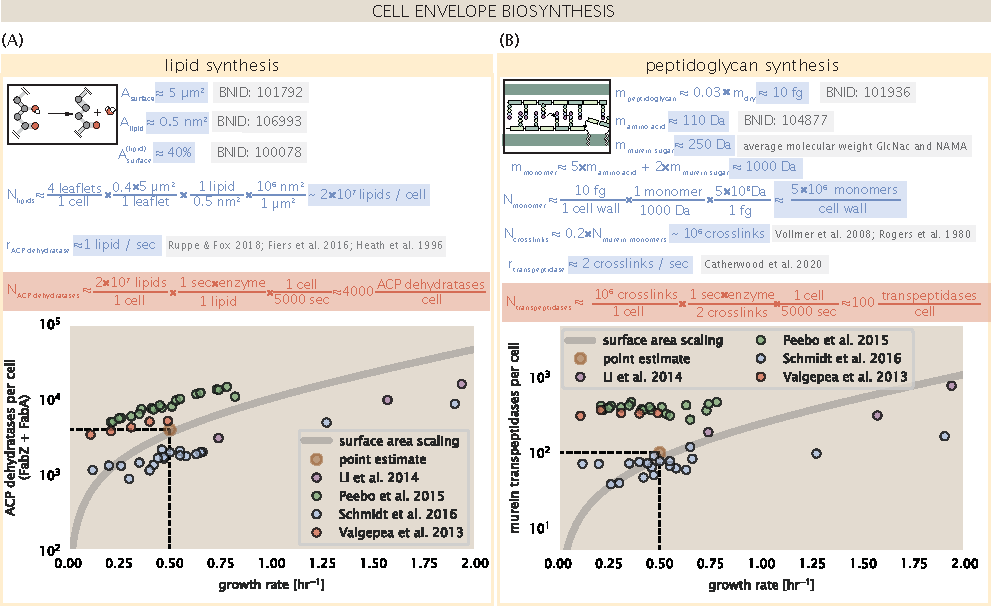
\includegraphics{main_figs/cell_wall_peptidoglycan.pdf}
    \caption{(A) Top panel shows an estimation for the
            number of ACP dehydratases necessary to form functional
            phospholipids, which is assumed to be a rate-limiting step on
            lipid synthesis. The rate of ACP dehydratases was inferred from
            experimental measurements via a stochastic kinetic model
            described in \cite{ruppe2018}. Bottom panel shows the
            experimentally observed complex copy numbers using the
            stoichiometries [FabA]$_2$ and [FabZ]$_2$. (B) An estimate for
            the number of peptidoglycan transpeptidases needed to complete
            maturation of the peptidoglycan. The mass of the murein monomer
            was estimated by approximating each amino acid in the
            pentapeptide chain as having a mass of 110 Da and each sugar in
            the disaccharide having a mass of $\approx$ 250 Da. The
            \textit{in vivo} rate of transpeptidation rein \textit{E. coli}
            was taken from recent analysis by \cite{catherwood2020}. The
            bottom panel shows experimental measurements of the
            transpeptidase complexes in \textit{E. coli} following the
            stoichiometries [MrcA]$_2$, [MrcB]$_2$, [MrdA]$_1$, and
            [MrdB]$_1$. Grey curves in each plot show the estimated number of
            complexes needed to satisfy the synthesis requirements scaled by
            the surface area as a function of growth
            rate.}
            \label{fig:cell_envelope}
    }
    \end{fullwidth}
\end{figure}
